 La velocidad del viento es una magnitud vectorial tridimensional que experimenta fluctuaciones aleatorias de pequeña escala en el espacio y en el tiempo, que se superponen a un flujo organizado de mayor escala. Para los fines de la observación meteorológica, la meteorología sinóptica y el pronóstico del tiempo, es crucial analizar el movimiento horizontal del aire que se define como viento. No obstante, es importante considerar que, para algunas aplicaciones, también es necesario conocer el movimiento vertical del viento. Ejemplos de esto son el aterrizaje de aeronaves y el estudio de la dispersión de contaminantes en la atmósfera. En la Figura \ref{fig:vectorVelocidad} se muestran las tres componentes de un vector de viento $\mathbf{v_{xyz}}$, y sobre el plano $XY$ se muestra la proyección $\mathbf{v_{xy}}$ que no interesa analizar.

\begin{figure}[H]
    \centering
    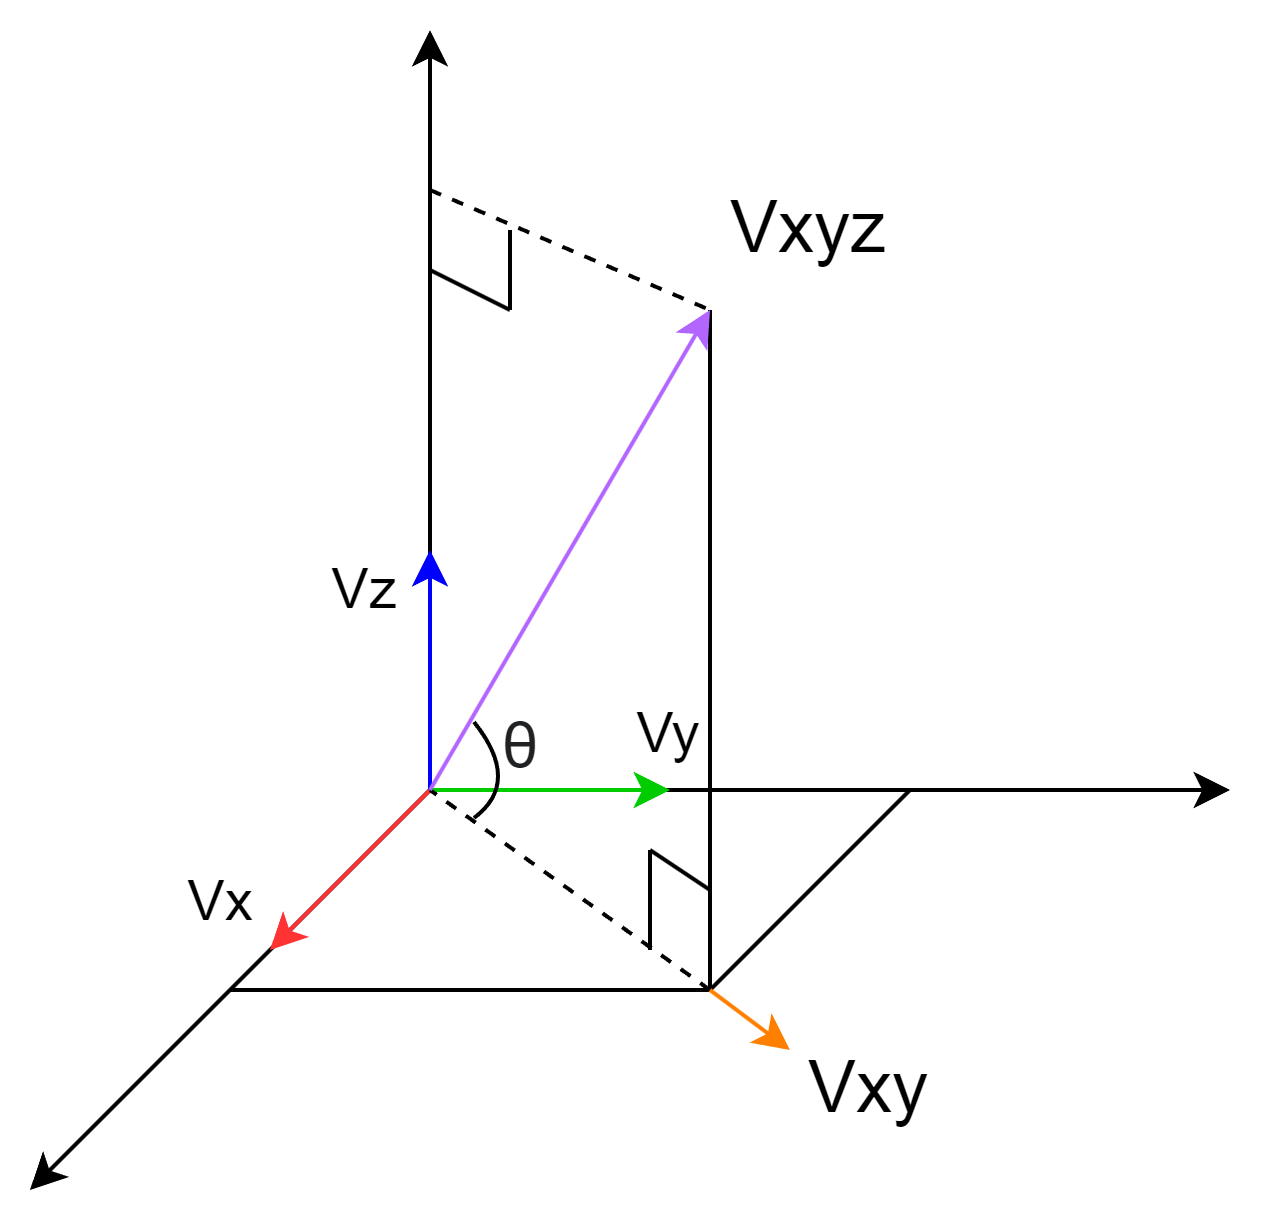
\includegraphics[width=0.5\linewidth]{Figuras/introduccion/vectorVelocidad.png}
    \caption{Tres componentes de la velocidad de viento $v_{x}, v_{y}, v_{z}\  [\frac{m}{s}]$. El vector de viento horizontal $v_{xy}$ forma un ángulo de entrada $\theta$ con el vector de viento resultante $v_{xyz}$.} 
    \label{fig:vectorVelocidad}
\end{figure}

\section{Viento en superficie}\label{sec:vientoEnSuperficie}
Se considerará que el viento de superficie es fundamentalmente una magnitud vectorial bidimensional definida por dos componentes
\begin{itemize}
    \item \textbf{Intensidad:} Indica el valor de la velocidad del viento. En general se utilizan unidades como nudos (\unit{\knot}), metros por segundo (\unit{\meter\per\second}) o kilómetros por hora (\unit{\kilo\meter\per\hour}).
    \item \textbf{Dirección y sentido:} Indica desde donde proviene el aire que se encuentra en movimiento. Se mide en grados sexagesimales y considera el apartamiento con respecto al norte geográfico. Por ejemplo, un viento de dirección noreste (aire que se desplaza del noreste hacia el suroeste) tiene una dirección de 45°, ya que esta es la separación (en grados) entre el norte y el noreste.
\end{itemize}

El grado de fluctuación experimentado por el viento se denomina  ráfagosidad, y las diferentes fluctuaciones son conocidas como ráfagas o rachas. La mayoría de los usuarios de datos sobre el viento necesitan conocer el viento horizontal en promedio, eliminando las fluctuaciones. Por ejemplo, en meteorología se utilizan promedios de entre 10 y 60 minutos con fines de predicción, mientras que en aeronáutica se utilizan promedios de 2 minutos. No obstante, cada vez son más las aplicaciones que precisan información acerca de la variabilidad o ráfagosidad del viento. Para este propósito, se utilizan tres magnitudes: la ráfaga o racha máxima, y las desviaciones típicas de la velocidad y de la dirección del viento \cite{wmoChapter8}.

La representación gráfica del viento se puede realizar de distintas formas, entre ellas se encuentran las flechas, las barbas y las líneas de corriente \cite{CursoDeObsevadores}.

Las \textbf{flechas} son la forma más común de representar un vector. La intensidad del viento se representa con la longitud de la flecha, mientras que la dirección se indica por el ángulo respecto al norte. El sentido de la flecha siempre apunta "hacia dónde va el viento". En la figura\footnote{Imagen extraída del curso de observadores \url{https://crf.smn.gob.ar/}} \ref{fig:mapaFlechas} se muestra un ejemplo en el que se observa que el viento en la Patagonia proviene principalmente del sector oeste (es decir, el aire se desplaza de oeste a este), por lo tanto, las flechas apuntan hacia el este.

\begin{figure}[H]
    \centering
    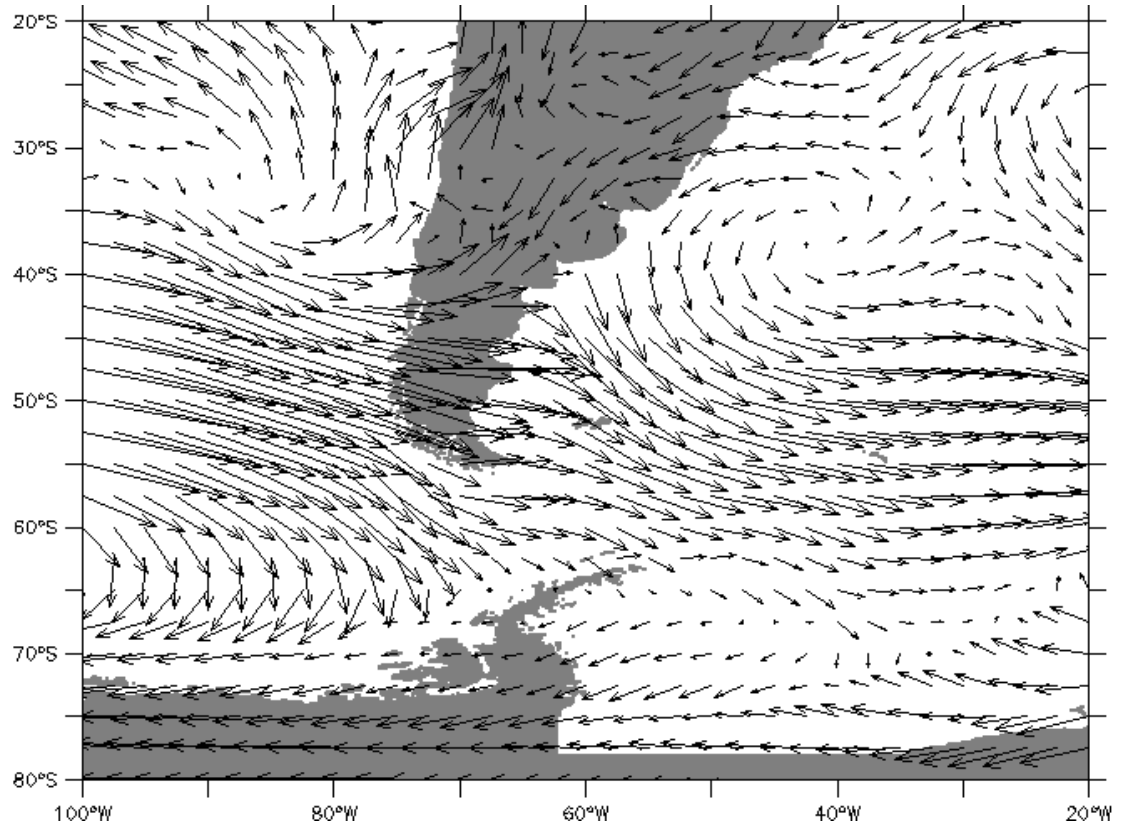
\includegraphics[width=0.85\linewidth]{Figuras/viento/mapaFlechas.png}
    \caption{Campo de viento representado con flechas en el sur de Sudamérica.}
    \label{fig:mapaFlechas}
\end{figure}

Las \textbf{barbas} son ideogramas en los que la línea más larga indica la dirección del viento, mientras que las líneas más pequeñas, ubicadas en un extremo, indican la intensidad en múltiplos de 5 \unit{knot}. En la figura \ref{fig:barbas1}, se puede observar una representación del viento del oeste con una intensidad de 15 nudos, donde la media flecha representa 5 \unit{knot} y la flecha entera representa 10 \unit{knot}. Más abajo, se observa una barba que representa el viento del sur con un banderín negro que indica una intensidad de 50 \unit{knot}. La dirección del viento está dada por el ángulo respecto al norte verdadero y, como se mencionó anteriormente, indica desde dónde viene el aire.

\begin{figure}[H]
    \centering
    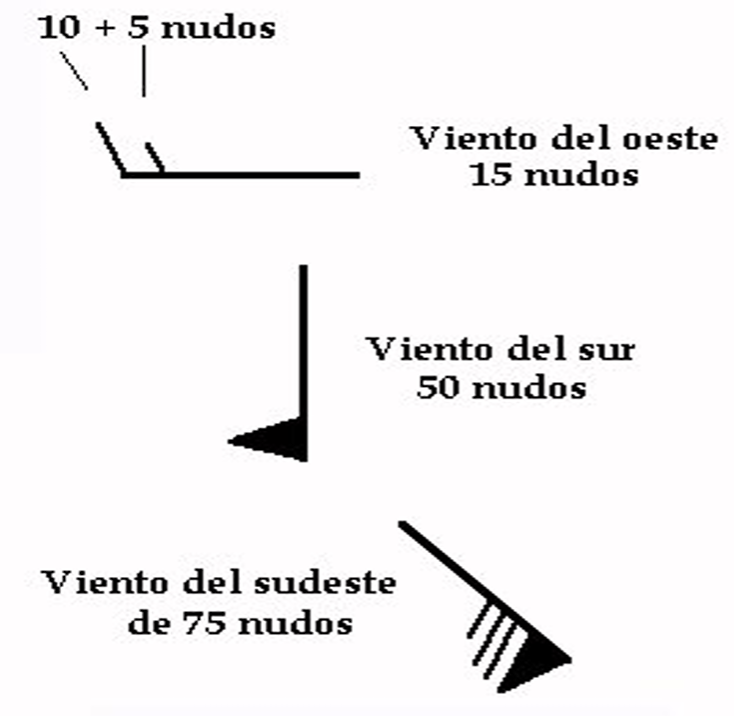
\includegraphics[width=0.4\linewidth]{Figuras/viento/barbas1.png}
    \caption{Representación gráfica del viento utilizando barbas.}
    \label{fig:barbas1}
\end{figure}
Las barbas son muy utilizadas en meteorología sinóptica y aeronáutica. En la figura\footnote{Imagen extraída del curso de observadores \url{https://crf.smn.gob.ar/}} \ref{fig:mapaBarbas} se muestra una representación gráfica del viento en 850 \unit{\hecto\pascal} utilizadas en la meteorología aeronáutica. Nótese en la elipse roja el viento de 40 \unit{knot} del sector oeste en el norte de la Patagonia, mientras que en la zona central del país prevalecen vientos del sector norte en torno a los 10 y 15 \unit{knot}.

\begin{figure}[H]
    \centering
    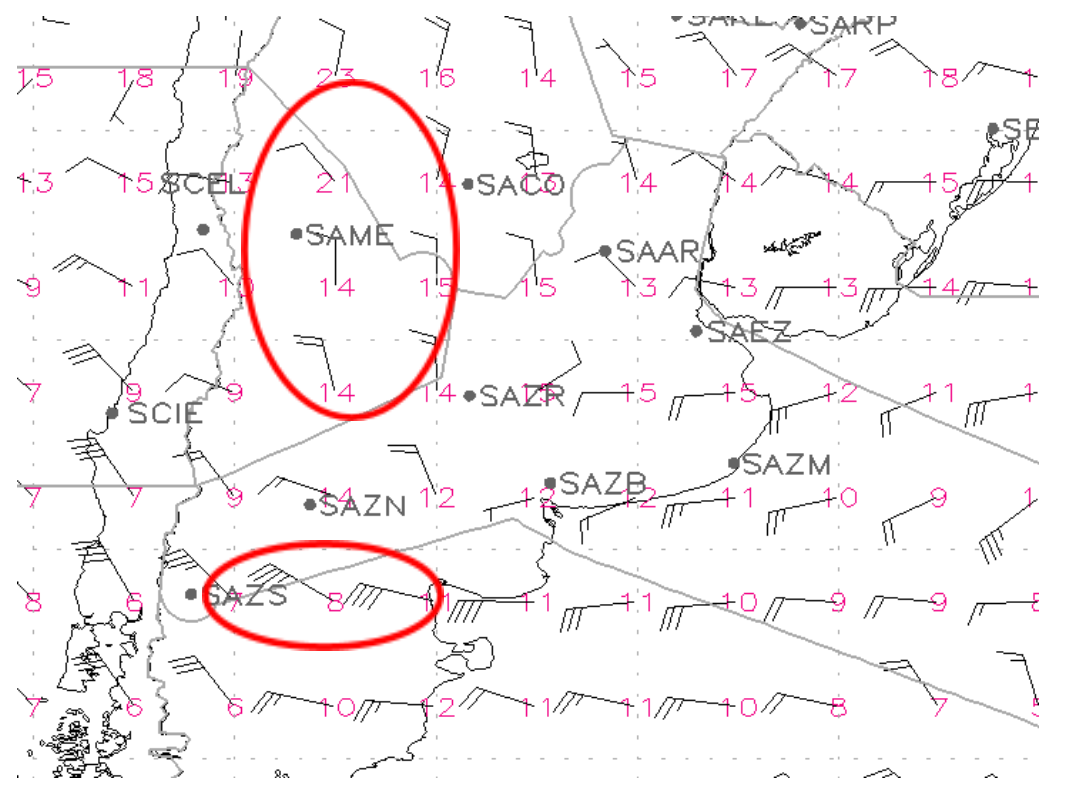
\includegraphics[width=0.85\linewidth]{Figuras/viento/mapaBarbas.png}
    \caption{Representación del viento en 850 \unit{\hecto\pascal} para el día 14/4/2016 a las 12 UTC en la región central de Argentina.}
    \label{fig:mapaBarbas}
\end{figure}

Las \textbf{Líneas de corriente} son la representación gráfica más utilizada para analizar los factores de la circulación a gran escala. Una línea de corriente se define como la curva cuya tangente en cualquiera de sus puntos tiene la dirección de la velocidad del aire. Se utilizan en general en niveles altos, así como también en superficie en zonas tropicales. Un ejemplo de esta representación se puede apreciar en la figura\footnote{Imagen extraída de la página del SMN \url{https://www.smn.gob.ar}}\ref{fig:mapaLineas}. En esta figura, se indica que un sistema de alta presión se desplazó al sur de la Patagonia argentina, lo que produjo el ingreso de aire templado a la península antártica, junto con condiciones de subsidencia que reforzaron aún más el efecto de secamiento y calentamiento del aire al descender hacia la superficie.

\begin{figure}[H]
    \centering
    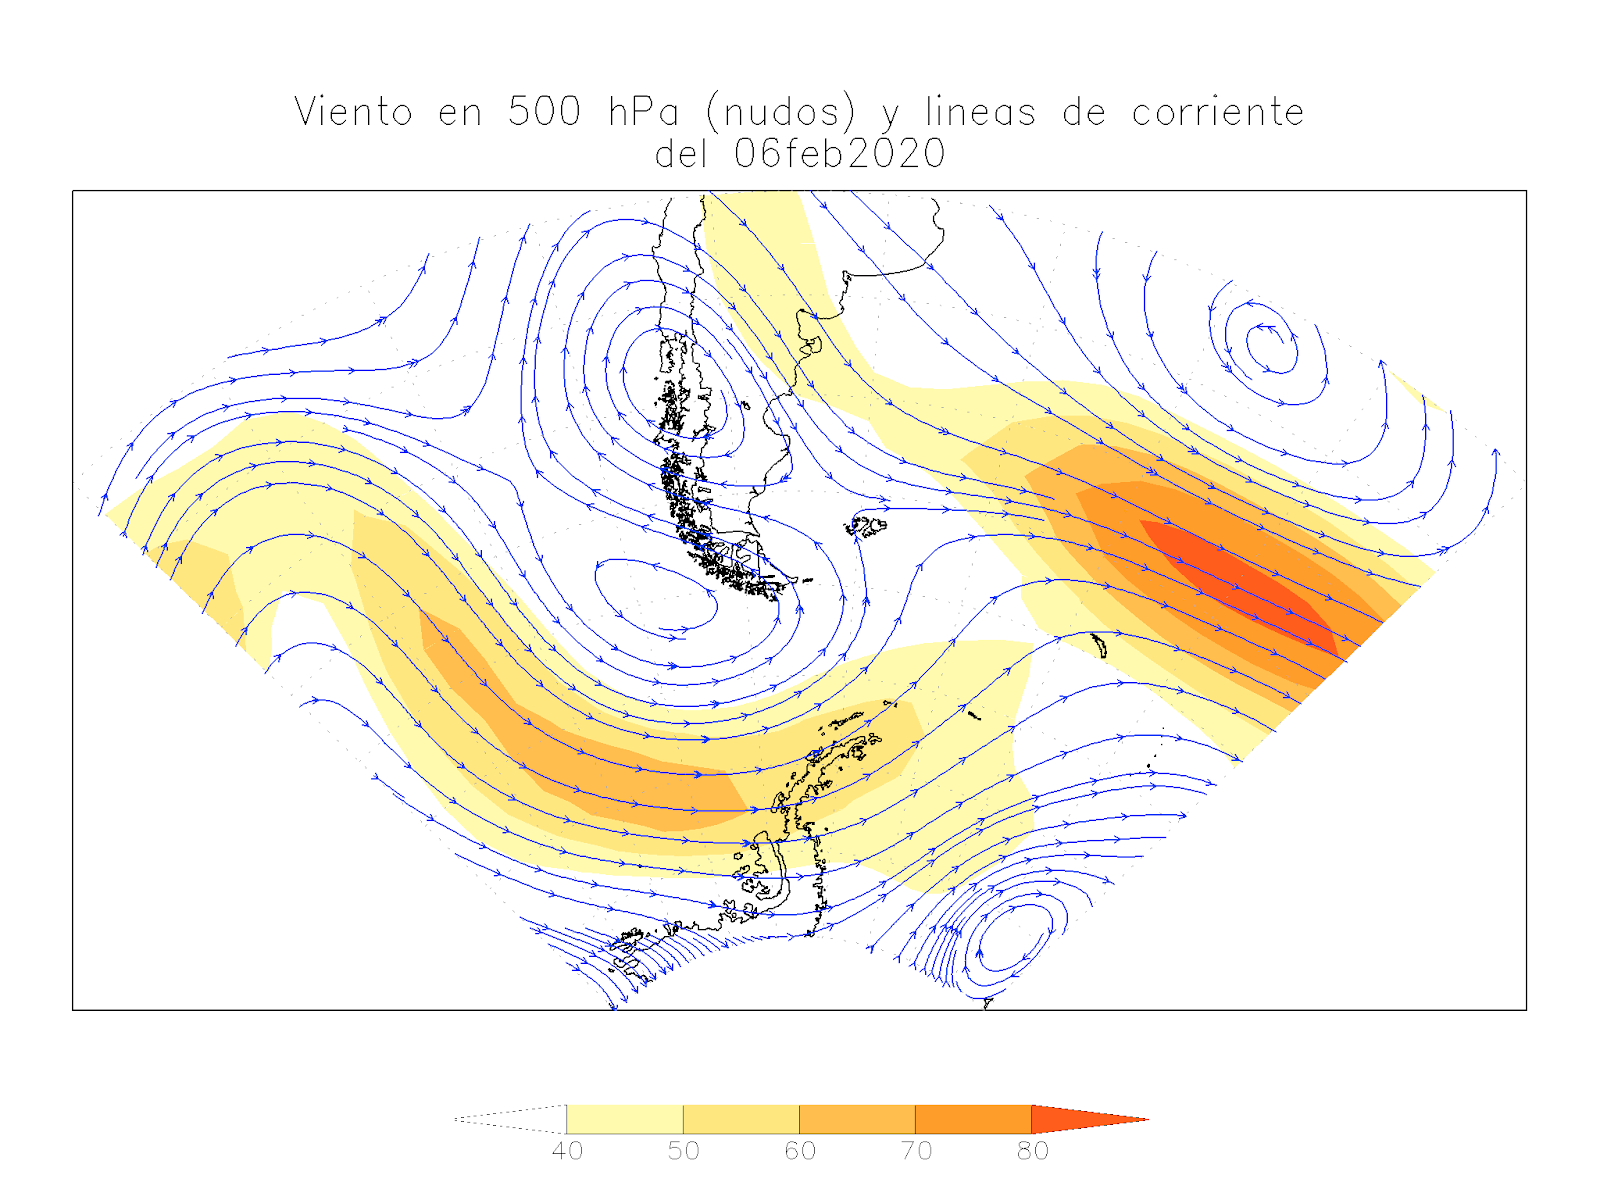
\includegraphics[width=1\linewidth]{Figuras/viento/mapalineasViento.png}
    \caption{Viento (nudos) y líneas de corriente en 500\unit{\hecto\pascal}.}
    \label{fig:mapaLineas}
\end{figure}


Si fuera necesario hablar de las fuerzas que actúan sobre el movimiento del aire

\section{Instrumentos de medición del viento}\label{sec:instrumentos_med_viento}
Aca dar el detalle de los manuales de Vaisala y DeltaOHM, como se mide el viento, sus partes y como se debe alinear en la instalacion, sacar todo de los manuales, mencionar por arriba la coperola, el anemo de hilo caliente y el laserdoplerlidar.



\section{Túnel de viento}

aca poner el modelo del patron utilizado en el tunel de viento

poner como mide viento el anemotro de ultrasonido con un esquema del manual del deltaOHM

\begin{figure}[H]
    \centering
    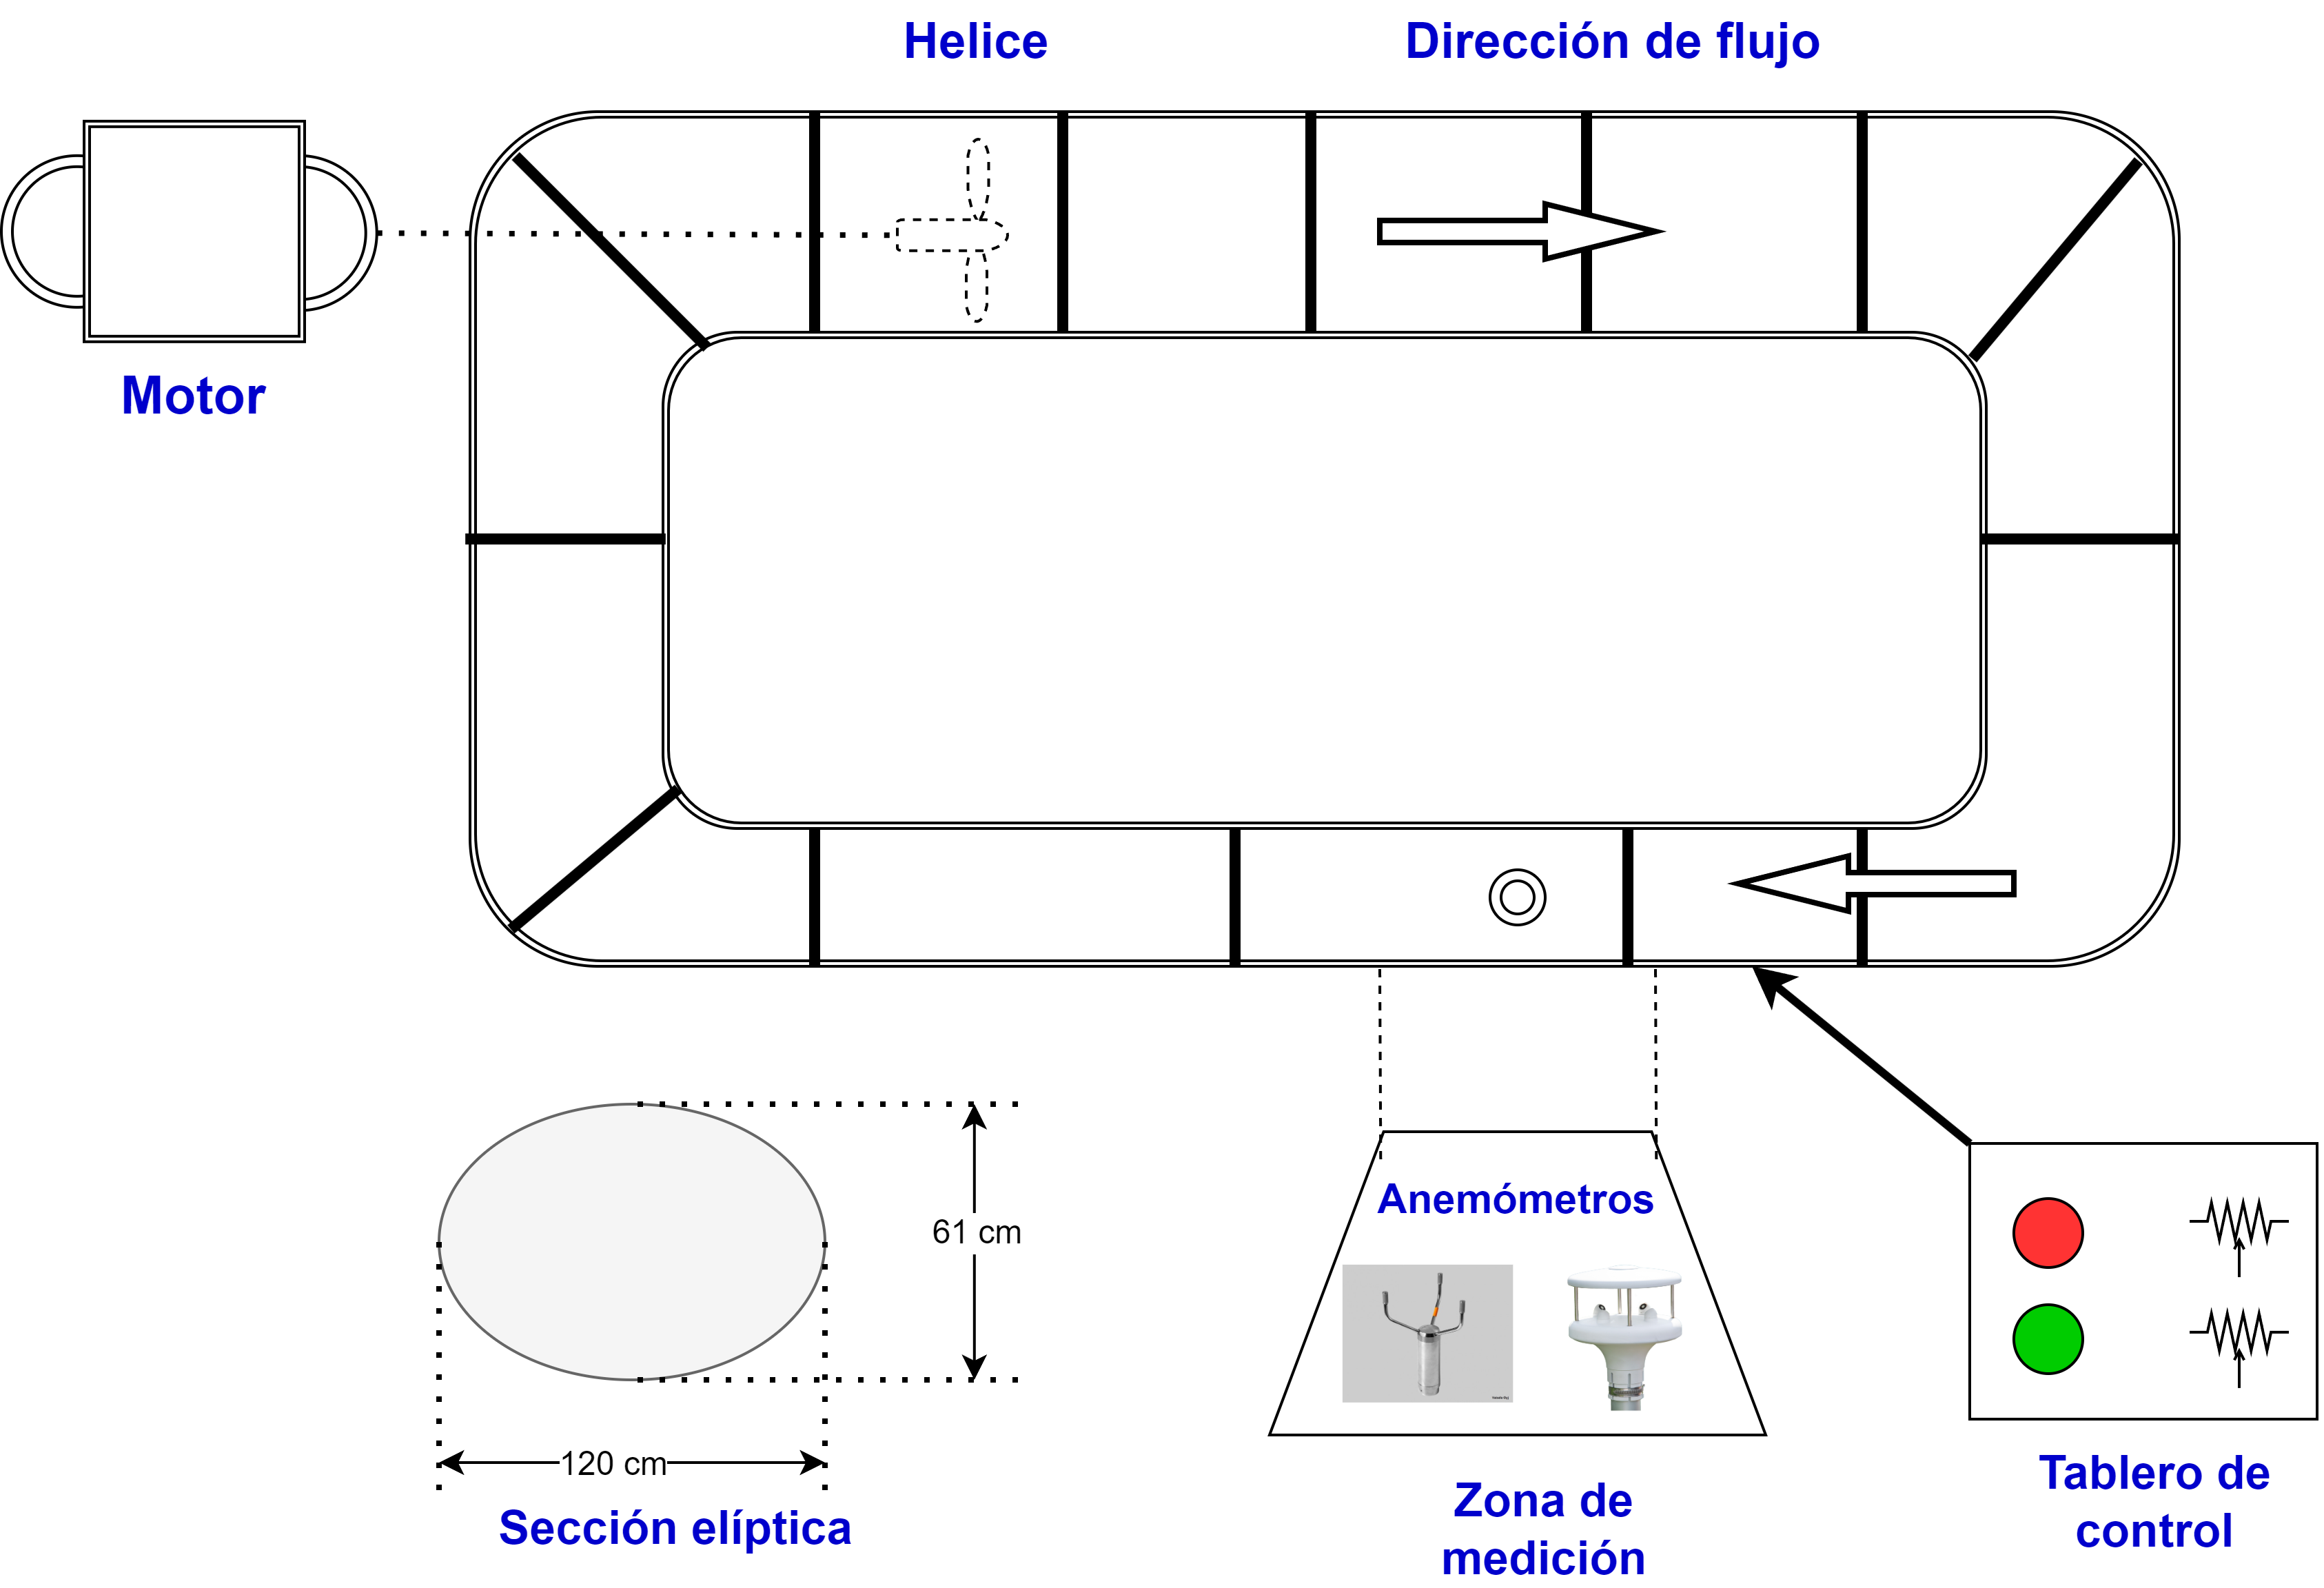
\includegraphics[width=1\linewidth]{Figuras/viento/TunelVientoEsquema.png}
    \caption{Túnel de viento.}
    \label{fig:tunelVientoEsquema}
\end{figure}

poner foto real del tunel de viento, zona de medicion, vista superior y del motor.
% \section{}